% 原书 p.55–p.62（PDF p.63–p.70）
\section{切触流形（Contact Manifold）}

\begin{keytakeaways}
\begin{itemize}
  \item 几何图像：标准切触结构 $\xi_{\mathrm{std}}=\ker(\dd z-y\,\dd x)$ 的 Reeb 流沿
        $z$ 方向平移；过扭切触结构 $\xi_{\mathrm{OT}}$ 沿 $r$-射线无限扭转；辛流形的
        切触型超曲面与单位余球面丛给出大批切触流形。
  \item 数学工具：Liouville 向量场（$L_Y\omega=\omega$）与 Liouville 域及其分解
        (3.10)、辛化 $SM=(\R\times M,\dd(e^r\alpha))$、切触化
        $CW=(W\times S^1,\ker(\lambda+\dd\theta))$。
  \item 本节结论：切触流形与辛流形经由辛化、切触化互相转化；单位余球面丛
        $(S^*_gQ,\lambda)$ 的闭 Reeb 轨道恰好对应于 $(Q,g)$ 的闭测地线；过扭结构
        在切触结构分类中居根本地位。
\end{itemize}
\end{keytakeaways}

% >>> p063
本节列举切触流形的若干基本例子，其中一些例子显示出辛流形与切触流形之间的紧密联系。

\begin{wexam}{3.2.1}（标准切触结构）
最基本的例子是欧氏空间 $\R^{2n+1}$，取坐标
$(x_1,\dots,x_n,y_1,\dots,y_n,z)$，并令
$\xi_{\mathrm{std}}:=\ker\alpha_{\mathrm{std}}$，其中
\begin{equation}\tag{3.3}
  \alpha_{\mathrm{std}}:=\dd z-\sum_{i=1}^n y_i\,\dd x_i .
\end{equation}
验证条件 (3.1)，可得
\[
  \alpha_{\mathrm{std}}\wedge(\dd\alpha_{\mathrm{std}})^n
  =\dd z\wedge\dd x_1\wedge\dd y_1\wedge\cdots\wedge\dd x_n
  \wedge\dd y_n\neq0 .
\]
由 (3.2)，$\alpha_{\mathrm{std}}$ 的 Reeb 向量场为
$R_{\alpha_{\mathrm{std}}}=\partial_z$。因此 Reeb 流就是沿 $z$ 方向的平移。图 3.2
逐点显示了 $(\R^3,\xi_{\mathrm{std}})$ 的切触结构，其中阴影「小片」局部表示
超平面场 $\xi$。注意，由于对任意常数平移 $c\in\R$ 都有 $\dd(z+c)=\dd z$ 与
$\dd(x+c)=\dd x$，超平面场 $\xi$ 在沿 $z$ 方向与沿 $x$ 方向平移下不变。同时，
在原点 $0\in\R^3$ 处有 $\xi=\langle\partial_x,\partial_y\rangle$。由此便可确定
$\R^3$ 中 $\xi$ 的绝大部分，只有沿 $y$ 方向移动时 $\xi$ 才会改变（旋转）。为研究
这一旋转，把任意 $v\in\xi$ 写成 $v=A\partial_x+B\partial_y+C\partial_z$，其中
$A,B,C$ 为待定系数。由 $\xi_{\mathrm{std}}=\ker\alpha_{\mathrm{std}}$ 可得
\[
  (\dd z-y\,\dd x)\left(A\frac{\partial}{\partial x}
  +B\frac{\partial}{\partial y}+C\frac{\partial}{\partial z}\right)=0,
\]
它等价于 $C-Ay=0$ 且 $B$ 任意。于是可取 $\xi$ 的一组基如下：
\[
  \xi_{(x,y,z)}=\bigl\langle\partial_x+y\,\partial_z,\ \partial_y\bigr\rangle .
\]
重要的是，沿 $y$ 轴移动时，相应的超平面旋转从不超过一整圈。\hfill$//$
\end{wexam}

% [Tutor Note: 易错预警——例 3.2.1 中「$\alpha\wedge(\dd\alpha)^n=\dd z\wedge
% \dd x_1\wedge\dd y_1\wedge\cdots$」应理解为「相差一个非零常数因子 $n!$」：
% 直接计算得 $(\dd\alpha_{\mathrm{std}})^n
% =(-\sum_i\dd y_i\wedge\dd x_i)^n=n!\,\dd x_1\wedge\dd y_1\wedge\cdots$，
% 再与 $\dd z$ 楔积即得。原文省略了 $n!$（$n=1$ 时恰为等式），核对时不要把它
% 当作逐项恒等式。另注意另一种常见约定是 $\alpha=\dd z+x\,\dd y$，形式不同但
% 切触结构同构，比较公式时须先对齐约定。]

% >>> p064
\begin{figure}[htbp]
  \centering
  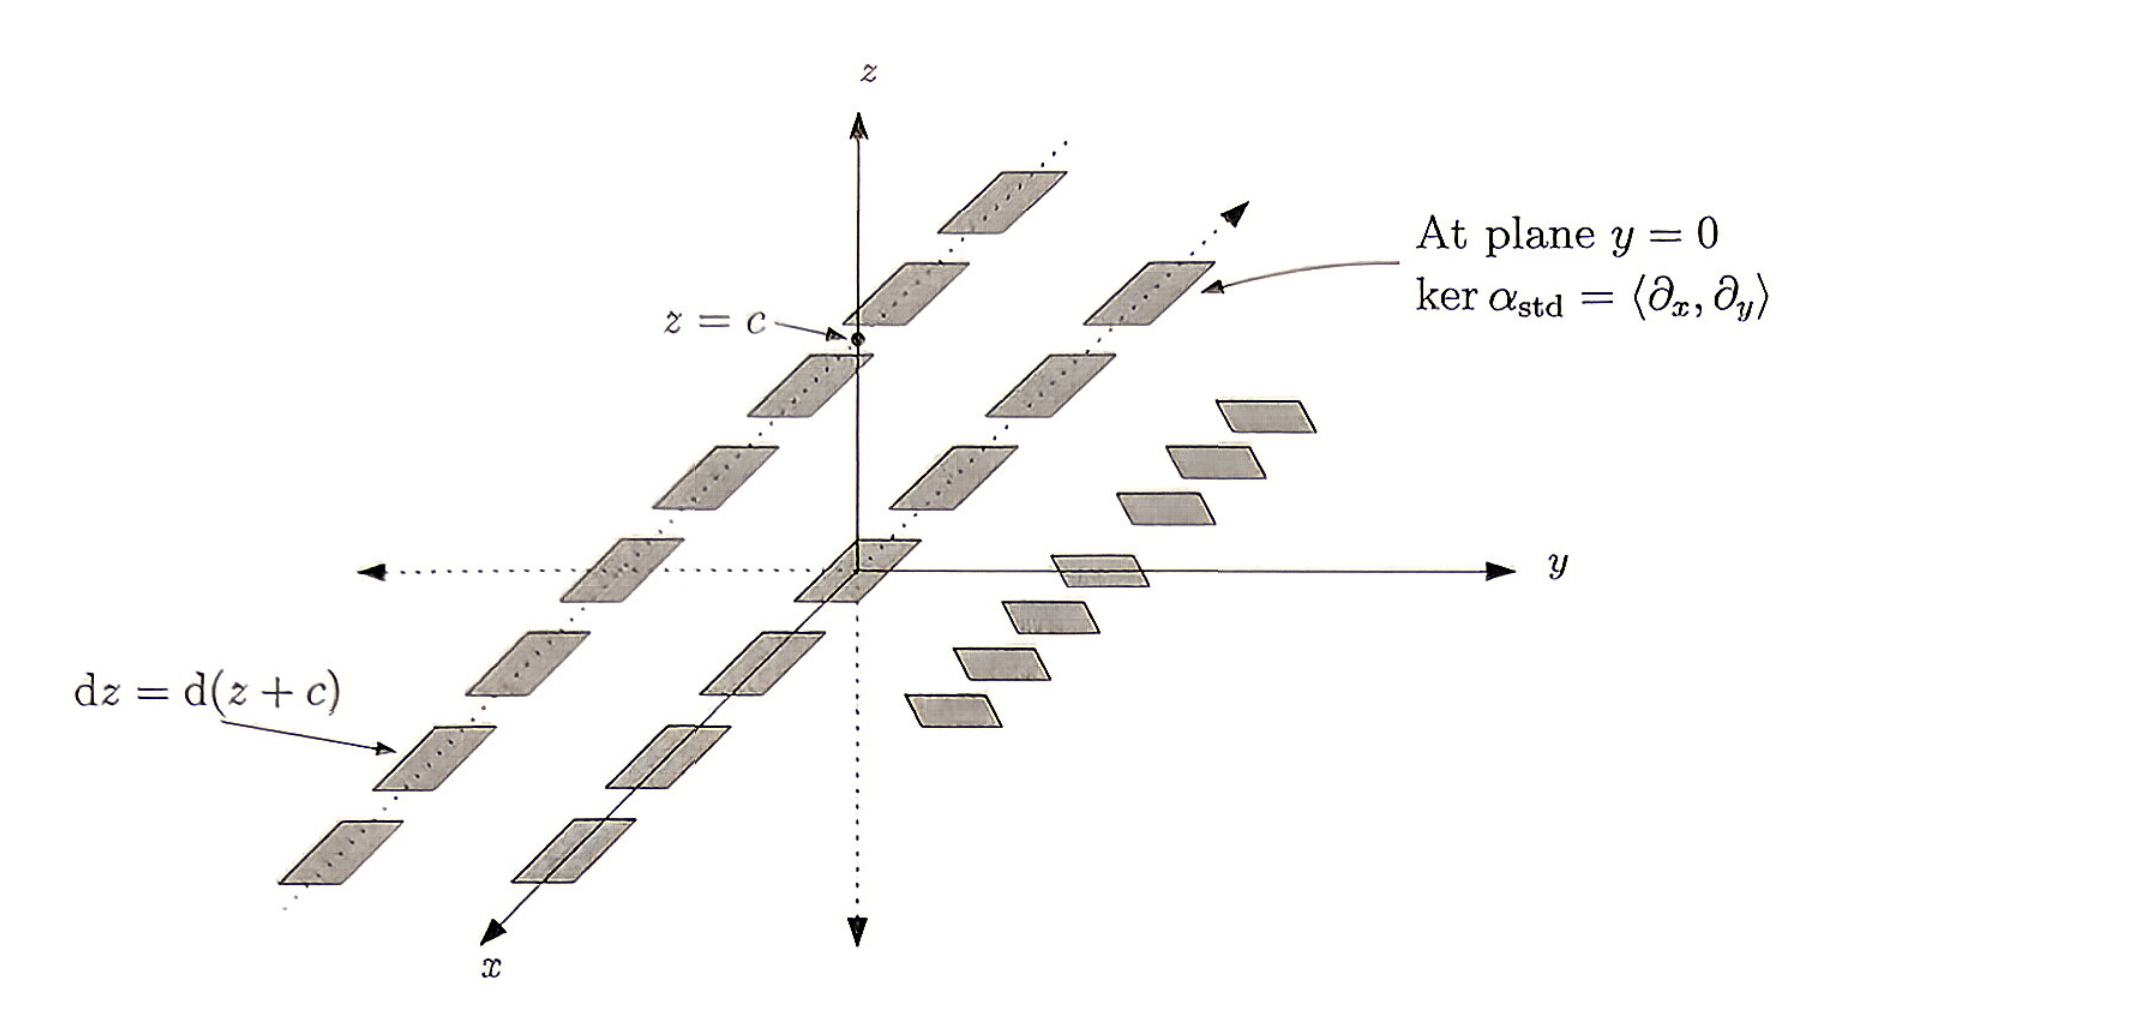
\includegraphics[width=0.62\linewidth]{figures/fig_p064_1.png}
  \caption*{图 3.2\quad $\R^3$ 上的标准切触结构 $\xi_{\mathrm{std}}$
  （原书 p.56, Figure 3.2）}
\end{figure}

\begin{wrem}{3.2.1}
除 (3.3) 定义的 $\alpha_{\mathrm{std}}$ 之外，通过对 $\alpha_{\mathrm{std}}$
作某些线性变换，还可得到 $\R^{2n+1}$ 上其他的切触形式。例如，文献中常出现
以下两种：
\[
  \alpha'=\dd z+\sum_{i=1}^n x_i\,\dd y_i,\qquad
  \alpha''=\dd z+\frac12\sum_{i=1}^n\bigl(x_i\,\dd y_i-y_i\,\dd x_i\bigr).
\]
不同的这类切触 $1$-形式可能给出不同的切触结构，但这些 $\xi$ 看上去与
$\xi_{\mathrm{std}}$ 大同小异，特别是不超过一整圈的扭转。
\end{wrem}

% [Tutor Note: 原文疑误——注 3.2.1 中「还可得到 $\R^n$ 上其他的切触形式」
% 应为「$\R^{2n+1}$」（本注中的 $\alpha'$、$\alpha''$ 显含 $x_i,y_i,z$ 共
% $2n+1$ 个坐标）。已记入 review_ch03.md。]

下一个例子展示欧氏空间中另一类切触结构。

\begin{wexam}{3.2.2}（过扭切触结构）
我们聚焦 $\R^3$，取柱坐标
$(r,\theta,z)\in\R_{\ge0}\times[0,2\pi)\times\R$。考虑如下 $1$-形式
\begin{equation}\tag{3.4}
  \alpha_{\mathrm{OT}}:=\cos r\,\dd z+r\sin r\,\dd\theta .
\end{equation}
容易验证 $\alpha_{\mathrm{OT}}$ 在 $r=0$ 之外满足非退化条件 (3.1)，因此
$\xi_{\mathrm{OT}}:=\ker\alpha_{\mathrm{OT}}$ 是
$\R^3\setminus\{r=0\}$ 上的切触结构。

与例 3.2.1 类似，我们想显式描述超平面场 $\xi_{\mathrm{OT}}$。注意
$\alpha_{\mathrm{OT}}$ 在坐标变换 $(r,\theta,z)\mapsto(r,\theta,z+c)$
（$c\in\R$）下不变，故沿 $z$ 方向移动时超平面场 $\xi$ 不变。一般地，把任意
$v\in\xi_{\mathrm{OT}}$ 写成 $v=A\partial_r+B\partial_\theta+C\partial_z$，
其中系数 $A,B,C$ 待定。于是
\[
  (\cos r\,\dd z+r\sin r\,\dd\theta)\left(A\frac{\partial}{\partial r}
  +B\frac{\partial}{\partial\theta}+C\frac{\partial}{\partial z}\right)=0,
\]
% >>> p065
它等价于 $\cos r\cdot C+r\sin r\cdot B=0$ 且 $A$ 任意。于是可取
$\xi_{\mathrm{OT}}$ 的如下一组基：
\[
  \xi_{\mathrm{OT}}=\Bigl\langle\cos r\frac{\partial}{\partial\theta}
  -r\sin r\frac{\partial}{\partial z},\ \frac{\partial}{\partial r}\Bigr\rangle .
\]
见图 3.3。

\begin{figure}[htbp]
  \centering
  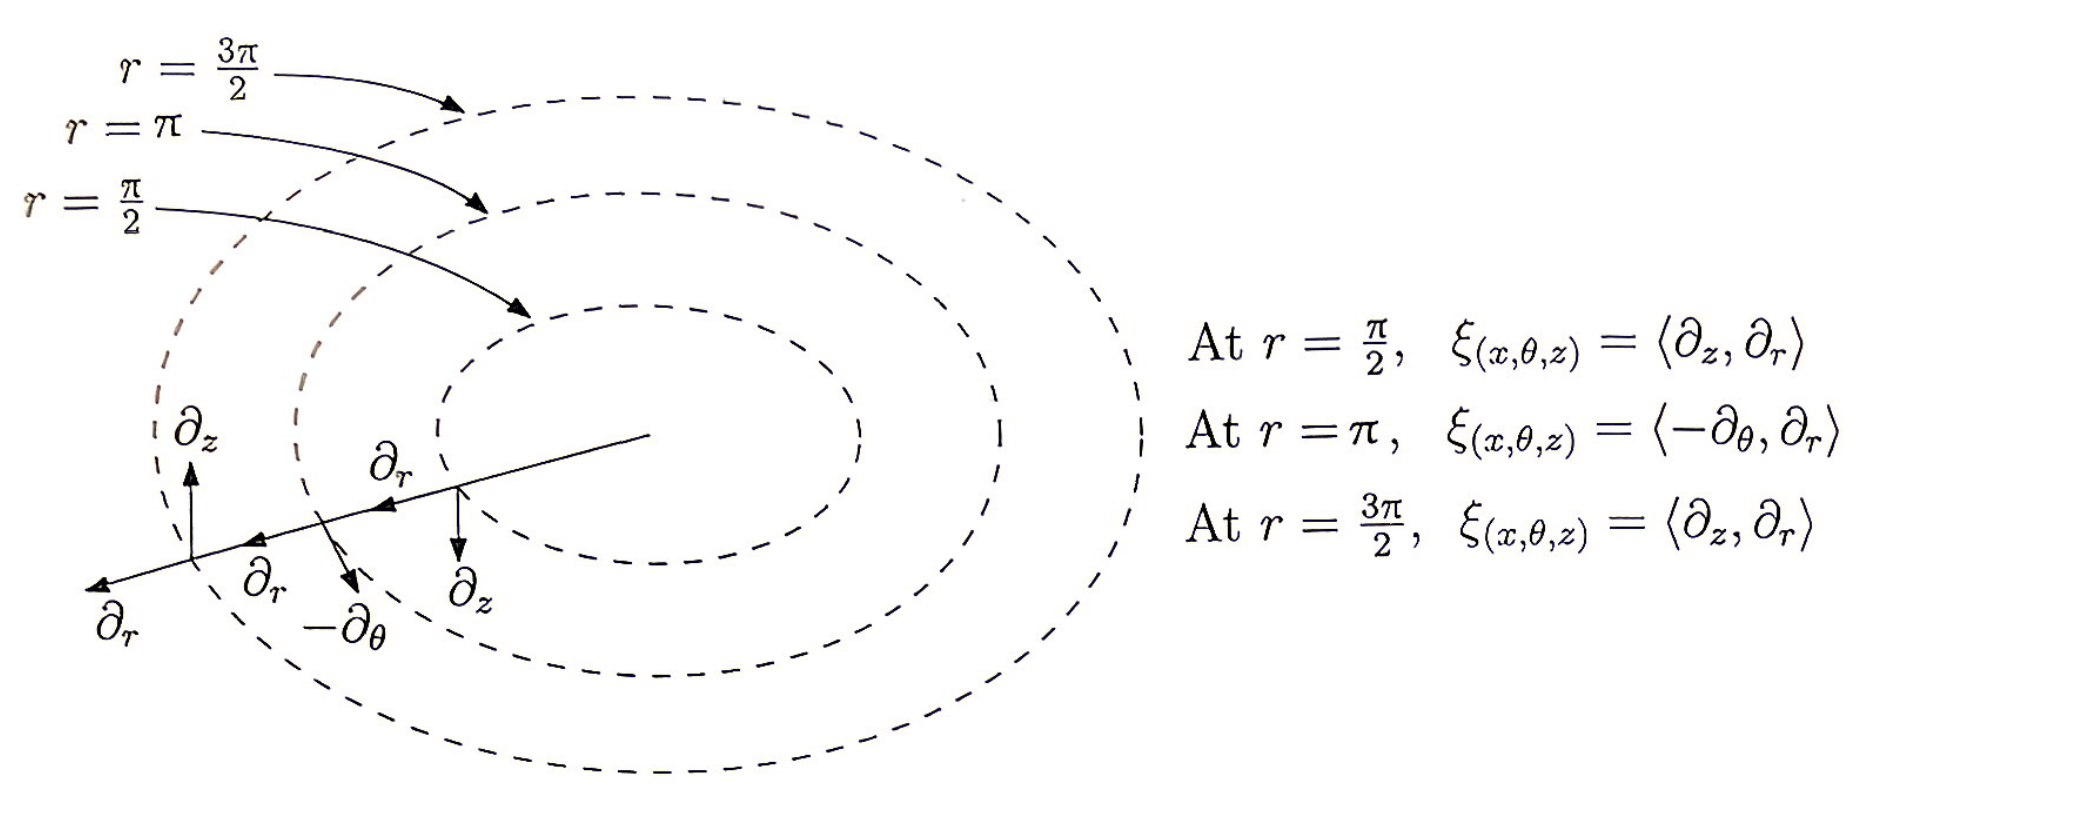
\includegraphics[width=0.78\linewidth]{figures/fig_p065_1.png}
  \caption*{图 3.3\quad $\R^3$ 中的过扭切触结构 $\xi_{\mathrm{OT}}$
  （原书 p.57, Figure 3.3）}
\end{figure}

注意基向量 $\cos r\,\partial_\theta-r\sin r\,\partial_z$ 在 $\theta z$-平面中
随角度 $r\in\R_{\ge0}$ 而旋转。特别地，沿任意 $r$-射线（朝 $r=\infty$）以任意
固定角 $\theta$ 移动时，相应的超平面会旋转无穷多次！正是由于这一现象，
$\R^3$ 中的这个切触结构 $\xi_{\mathrm{OT}}$ 被称为\textbf{过扭的}
（overtwisted）。\hfill$//$
\end{wexam}

% [Tutor Note: 术语依据与原文疑误——overtwisted 的通行译名为「过扭的」，与
% tight「紧的」相对；注意 tight 的「紧」与 compact 的「紧」同字不同义，须靠
% 上下文区分。另注意图 3.3 右侧标注写作 $\xi_{(x,\theta,z)}$，但本例取柱坐标
% $(r,\theta,z)$，按上下文应读作 $\xi_{(r,\theta,z)}$，原图印作
% $(x,\theta,z)$ 疑为笔误；译文保留原图、不改原图。已记入 review_ch03.md。]

\begin{wrem}{3.2.2}
切触结构 $\xi$ 在 $M$ 中\textbf{过扭}的正式定义是：存在（拓扑）圆盘
$D\subset M$，使其边界的切空间 $T\partial D$ 落在 $\xi$ 中。在例 3.2.2 中，
只需取圆盘 $\{(r,\theta,z)\in\R^3\mid0\le r\le\pi\}$。由于 Eliashberg [74]
（三维切触流形）以及 Borman–Eliashberg–Murphy [31]（高维切触流形）的革命性
工作，过扭切触结构在切触结构的分类中起着根本性的作用。
\end{wrem}

% [Tutor Note: 含糊点拨——过扭判据中「$T\partial D\subset\xi$」需沿整个边界
% $\partial D$ 成立。对圆盘 $r\le\pi$：边界为 $r=\pi$ 的圆周，其切向为
% $\partial_\theta$；而由上面的基，在 $r=\pi$ 处
% $\xi=\langle-\partial_\theta,\partial_r\rangle$，恰包含 $\partial_\theta$，
% 故该圆盘见证过扭。这与沿 $r$ 的无限扭转是同一现象的两面。]

下一个例子给出从一类特殊的辛流形系统地构造切触流形的方法。

\begin{wexam}{3.2.3}（切触型超曲面）
设 $(W^{2n},\omega)$ 是带边界的 $2n$ 维辛流形，并设边界 $\partial W$ 光滑。
假设在 $\partial W$ 的某个管状邻域 $U$ 内存在向量场 $Y$，满足以下两个条件：
\begin{enumerate}[label=(\roman*)]
  \item 向量场 $Y$ 指向外侧，且横截于 $\partial W$；
  \item 向量场 $Y$ 是 \textbf{Liouville 向量场}，即 $L_Y\omega=\omega$
        （这本质上意味着 $Y$ 的流共形地改变 $\omega$）。
\end{enumerate}
则我们断言：$\partial W$ 是 $(2n-1)$ 维切触流形，其切触结构为
$\xi=\ker(\iota_Y\omega|_{\partial W})$。为简洁起见，记
$\lambda=\iota_Y\omega|_{\partial W}$。为说明 $\lambda$ 确为切触 $1$-形式
（满足非退化条件 (3.1)），把 $\lambda$ 改写为
\begin{equation}\tag{3.5}
  \lambda=\iota_Y\omega|_{\partial W}=i^*(\iota_Y\omega),
\end{equation}
其中 $i$ 是 $\partial W$ 到 $U$ 的嵌入。又由上面条件 (ii)，
$\omega=L_Y\omega=\dd\iota_Y\omega+\iota_Y\dd\omega=\dd\iota_Y\omega$。于是
有下述计算：
\begin{equation}\tag{3.6}
\begin{aligned}
  \lambda\wedge(\dd\lambda)^{n-1}
  &=i^*(\iota_Y\omega)\wedge\bigl(i^*(\dd\iota_Y\omega)\bigr)^{n-1}\\
  &=i^*(\iota_Y\omega)\wedge i^*(\omega^{n-1})
   =i^*\bigl(\iota_Y\omega\wedge\omega^{n-1}\bigr).
\end{aligned}
\end{equation}
% >>> p066
由上面条件 (i)，在每点 $x\in\partial W$ 处存在 $T_xW$ 的基
$\{e_1,\dots,e_{2n}\}$，其中 $e_{2n}=Y$，而 $\{e_1,\dots,e_{2n-1}\}$ 是
$T_x\partial W$ 的基。于是 $(\omega(x))^n(e_1,\dots,e_{2n-1},Y)\neq0$
（因 $\omega$ 是辛结构）蕴含
$(\iota_Y\omega\wedge\omega^{n-1})(e_1,\dots,e_{2n-1})\neq0$。

现在把上述构造应用于 $\R^4$（$\cong\C^2$）中的区域；对
$\R^{2n}$（$\cong\C^n$）有类似的讨论。实维数为 $4$ 的\textbf{辛椭球}
（symplectic ellipsoid）定义如下：
\begin{equation}\tag{3.7}
  E(a,b):=\Bigl\{(z_1,z_2)\in\C^2
  \ \Big|\ \frac{|z_1|^2}{a}+\frac{|z_2|^2}{b}\le1\Bigr\},
\end{equation}
其中辛形式 $\omega=\omega_{\mathrm{std}}$ 继承自
$(\R^4,\omega_{\mathrm{std}})$。把坐标识别为
$(z_1,z_2)=(x_1,y_1,x_2,y_2)$，并考虑由下式定义的\textbf{径向向量场}：
\begin{equation}\tag{3.8}
  Y_{(z_1,z_2)}:=\frac12\left(x_1\frac{\partial}{\partial x_1}
  +y_1\frac{\partial}{\partial y_1}+x_2\frac{\partial}{\partial x_2}
  +y_2\frac{\partial}{\partial y_2}\right).
\end{equation}
容易验证 $Y$ 横截于 $\partial E(a,b)$，即满足上面条件 (i)。又由条件 (ii)，
\begin{align*}
  L_Y\omega_{\mathrm{std}}
  &=\dd\iota_Y\omega_{\mathrm{std}}
   =\dd\iota_Y(\dd x_1\wedge\dd y_1+\dd x_2\wedge\dd y_2)\\
  &=\frac12\,\dd\bigl(x_1\dd y_1-y_1\dd x_1+x_2\dd y_2-y_2\dd x_2\bigr)\\
  &=\frac12\bigl(\dd x_1\wedge\dd y_1-\dd y_1\wedge\dd x_1
   +\dd x_2\wedge\dd y_2-\dd y_2\wedge\dd x_2\bigr)
   =\omega_{\mathrm{std}}.
\end{align*}
因此 $(\partial E(a,b),\iota_Y\omega_{\mathrm{std}}|_{\partial E(a,b)})$ 是
切触流形。

结束本例之前，我们要强调 $\partial E(a,b)$ 上的 Reeb 向量场计算如下：
\[
  R_\lambda=-\frac{2y_1}{a}\frac{\partial}{\partial x_1}
  +\frac{2x_1}{a}\frac{\partial}{\partial y_1}
  -\frac{2y_2}{b}\frac{\partial}{\partial x_2}
  +\frac{2x_2}{b}\frac{\partial}{\partial y_2},
\]
% >>> p067
其中沿用上面的记号 $\lambda=\iota_Y\omega_{\mathrm{std}}|_{\partial E(a,b)}$。
特别地，Reeb 流的行为如下：对任意 $(z_1,z_2)\in\partial E(a,b)$，
\begin{equation}\tag{3.9}
  \varphi^t_{R_\lambda}(z_1,z_2)
  =\bigl(\ee^{(2\sqrt{-1}/a)t}z_1,\ \ee^{(2\sqrt{-1}/b)t}z_2\bigr),
  \qquad t\in\R .
\end{equation}
为描述该 Reeb 流的闭轨道，分两种情形：
\begin{enumerate}[label=(\roman*)]
  \item 若 $a/b$ 有理，则从任意 $(z_1,z_2)\in\partial E(a,b)$ 出发都得到闭轨道。
        特别地，当 $a=b$（此时 $E(a,a)=:B^4(a)$，即 $4$ 维辛球）时，(3.9) 中的
        流描述的正是经典的 Hopf 纤维化；
  \item 若 $a/b$ 无理，则只有两条\textbf{单的}（simple）闭 Reeb 轨道（单的，
        或更常称为\textbf{素的}（prime），意指它们不是其他轨道的迭代），对应于
        圆周
        \[
          \gamma_a:=\{(z_1,0)\in\partial E(a,b)\mid |z_1|=a\},\qquad
          \gamma_b:=\{(0,z_2)\in\partial E(a,b)\mid |z_2|=b\},
        \]
        其周期分别为 $\pi a$ 与 $\pi b$。
\end{enumerate}

  \hfill$//$
\end{wexam}

% [Tutor Note: 原文疑误——按 (3.7) 中 $E(a,b)$ 的定义，在 $\partial E(a,b)$ 上
% 取 $z_2=0$ 得 $|z_1|^2=a$，故应为 $|z_1|=\sqrt a$（同理
% $|z_2|=\sqrt b$），而原文两处写的是 $|z_1|=a$、$|z_2|=b$。两种写法给出的
% 周期仍是 $\pi a$、$\pi b$（与 (3.9) 中 $2\sqrt{-1}/a$ 一致），故原文只在
% 半径处笔误。译文保留原文写法，已记入 review_ch03.md。]

例 3.2.3 中考虑的辛流形 $(W,\omega)$ 只容许在 $\partial W$ 的某个管状邻域内
定义向量场 $Y$。若 $Y$ 在整个 $(W,\omega)$ 上都存在，则称 $(W,\omega)$ 为
\textbf{Liouville 域}（Liouville domain）。而且，整体定义的 $Y$ 会大大简化
$(W,\omega)$ 的结构。事实上，对任意 Liouville 域有如下分解：
\begin{equation}\tag{3.10}
  W=\Bigl(\bigcup_{t\le0}\varphi^t_Y(\partial W)\Bigr)\sqcup
  \Op{Core}(W,\omega),
\end{equation}
其中 $\varphi^t_Y$ 表示 $Y$ 的流，$\Op{Core}(W,\omega)$ 一般是 $W$ 的子集
（称为 $(W,\omega)$ 的\textbf{核}（core））。当然，也可以通过补入流
$\varphi^t_Y$ 在 $t\ge0$ 时的像来「完备化」(3.10) 中的分解。几何上，补入
这样一个大的「端」，就把 Liouville 域 $(W,\omega)$ 完备化为一个非紧辛流形，
通常记为 $(\widehat W,\widehat\omega)$，并称为 $(W,\omega)$ 的
\textbf{完备化}（completion）。例如，在例 3.2.3 的辛椭球 $E(a,b)$ 情形，
(3.8) 中定义的径向向量场 $Y$ 是整体定义的，且
$\Op{Core}(E(a,b),\omega_{\mathrm{std}})=\{0\}$，其完备化为
$(\widehat{E(a,b)},\widehat{\omega_{\mathrm{std}}})=(\C^n,\omega_{\mathrm{std}})$。

% [Tutor Note: 含糊点拨——(3.10) 中 $\Op{Core}(W,\omega)$ 的确切含义是
% $\bigcap_{t\le0}\varphi^t_Y(W)$，即其逆向流（$t\to-\infty$）始终留在 $W$
% 内的点集；它与「$t\le0$ 时边界的流像的并」互补，构成 $W$ 的不交并分解。
% 教材只说它「一般是子集」，未给出定义，做习题时须自行补上。注意 $t\ge0$
% 的流像会跑出 $W$，故分解只能取 $t\le0$ 一侧。]

下一个例子给出另一类有用的 Liouville 域，它与黎曼几何密切相关。

\begin{wexam}{3.2.4}
设 $(Q,g)$ 是 $n$ 维黎曼流形，度量为 $g$。考虑余切丛 $T^*Q$ 的如下区域：
\begin{equation}\tag{3.11}
  D^*_gQ:=\bigl\{(q,p)\in T^*Q \ \big|\ \|p\|_{g^*}\le1\bigr\},
\end{equation}
% >>> p068
其中 $g^*$ 是 $T^*Q$ 上的对偶度量。$T^*Q$ 上的典范辛结构
$\omega_{\mathrm{can}}$ 限制到 $D^*_gQ$ 上仍为辛结构，因此
$(D^*_gQ,\omega_{\mathrm{can}})$ 是带边界的辛流形，称为 $(Q,g)$ 的
\textbf{单位余圆盘丛}（unit codisk bundle）。应用例 3.2.3，取局部由
$p\,\partial_p$ 定义的向量场 $Y$。对任意 $(q,p)\in D^*_gQ$，向量
$Y_{(q,p)}$ 指向外侧且横截于边界
$\partial D^*_gQ=\{(q,p)\in D^*_gQ\mid\|p\|_{g^*}=1\}$。同时可验证
\[
  L_Y\omega_{\mathrm{can}}=\dd\iota_Y\omega_{\mathrm{can}}
  =\dd\bigl((\dd p\wedge\dd q)(p\,\partial/\partial p,\cdot)\bigr)
  =\dd p\wedge\dd q=\omega_{\mathrm{can}}.
\]
于是例 3.2.3 的两个条件均满足，这说明 $Y_{(q,p)}$ 是 Liouville 向量场，且
$(\partial D^*_gQ,\iota_Y\omega_{\mathrm{can}}|_{\partial D^*_gQ})$ 是
切触流形。

为简洁起见，记
\begin{equation}\tag{3.12}
  (S^*_gQ,\lambda):=
  \bigl(\partial D^*_gQ,\iota_Y\omega_{\mathrm{can}}|_{\partial D^*_gQ}\bigr),
\end{equation}
称之为 $(Q,g)$ 的\textbf{单位余球面丛}（unit cosphere bundle）。我们来研究
$(S^*_gQ,\lambda)$ 上相应的 Reeb 向量场 $R_\lambda$。考虑由哈密顿函数
$H(q,p)=\frac12\|p\|^2_{g^*}$（$(q,p)\in T^*Q$）生成的哈密顿向量场 $X_H$。
特别地，$S^*_gQ=H^{-1}(0.5)$。注意对 (3.12) 中的 $\lambda$，有
\begin{equation}\tag{3.13}
  \lambda(X_H|_{S^*_gQ})=(\iota_Y\omega_{\mathrm{can}})(X_H)
  =\dd H(Y)=\|p\|^2_{g^*}=1.
\end{equation}
同时，由于 $\dd\lambda=\omega_{\mathrm{can}}$，限制到 $S^*_gQ$ 上有
\[
  \dd\lambda(X_H,\cdot)=\omega_{\mathrm{can}}(X_H,\cdot)
  =-\dd H(\cdot)=0,
\]
其中最后一个等号来自 $H|_{S^*_gQ}=1/2$。于是按定义，
$X_H|_{S^*_gQ}$ 就是 $(S^*_gQ,\lambda)$ 的 Reeb 向量场 $R_\lambda$。此外，
练习 2.2.1 的解答与例 2.1.2 表明：在相差一个 Legendre 变换的意义下，求解
$X_H$（限制在 $S^*_gQ$ 上）的哈密顿系统等价于求解测地线的拉格朗日系统。
因此可以断定：$(S^*_gQ,\lambda)$ 的闭 Reeb 轨道恰对应于 $(Q,g)$ 的闭测地线。\hfill$//$
\end{wexam}

\begin{wrem}{3.2.3}（与 D. Cant 的交流）
对照例 3.2.3 与例 3.2.4 中切触流形的构造，关键要素是向量场 $Y$（在例 3.2.3
中 $Y$ 是 (3.8) 中的径向向量场；在例 3.2.4 中 $Y=p\partial_p$），而不是切触
$1$-形式 $\lambda$（它可由 $\iota_Y\omega$ 导出）。此外，注意到 Liouville 域
$(W,\omega)$ 中的定义向量场 $Y$ 可以延拓为完备化
$(\widehat W,\widehat\omega)$ 上良定义的 Liouville 向量场 $Y$。这启发了另一条
从辛流形得到切触流形的途径。

确切地说，考虑一个\textbf{非紧}辛流形 $(X,\omega)$，它容许整体定义的
Liouville 向量场 $Y$（同样在 $L_Y\omega=\omega$ 的意义下）——这样的流形称为
\textbf{Liouville 流形}（Liouville manifold）。
\end{wrem}

% >>> p069
记 $\varphi^t_Y$ 为 $Y$ 的流。按分解 (3.10)，在补集
$X\setminus\Op{Core}(X,\omega)$ 上有一个 $\R$-作用，具体为
$s\cdot x\mapsto\varphi^s_Y(x)$（$s\in\R$）。事实上可以证明，商空间
$(X\setminus\Op{Core}(X,\omega))/\R$ 是一个流形，记为 $M$，且其上有切触
结构 $\xi$。这个切触流形 $(M,\xi)$ 称为\textbf{$(X,\omega)$ 关于 $Y$ 的理想
边界}（ideal boundary）（见 [176] 中例 1.12 正上方的段落）。作为例子，对
$(X,\omega)=(\C^n,\omega_{\mathrm{std}})$，其关于径向向量场 $Y$ 的理想边界
在拓扑上是 $S^{2n-1}$，并带有典范定义的切触结构 $\xi$（这与
$(X,\omega)=(T^*Q,\omega_{\mathrm{can}})$ 的情形类似）。换言之，尽管辛椭球
$E(a,b)$ 与辛球 $B^4(c)$ 的边界由 $\iota_Y\omega_{\mathrm{std}}$ 的限制得到
两个不同的切触 $1$-形式，但它们的核实际上给出同一个切触结构。

一般而言，把理想边界 $(M,\xi)$ 几何地实现为 $X$ 中某个显式区域的边界，等价于
在 $(M,\xi)$ 上固定一个切触 $1$-形式，这也等价于取如下投影的一个截面 $s$：
$\pi:X\setminus\Op{Core}(X,\omega)\to M$。

由上述讨论容易看出：Liouville 流形 $(X,\omega)$ 与 Liouville 流形
$(W,\omega)$ 通过完备化 $(\widehat W,\widehat\omega)=(X,\omega)$ 相联系，而
$(\partial W,\xi=\ker(\iota_Y\omega|_{\partial W}))$ 可看作截面
$s:M\to X\setminus\Op{Core}(X,\omega)$。特别地，这意味着（非紧）辛流形
$(X\setminus\Op{Core}(X,\omega),\omega)$ 不过是切触流形
$(\partial W,\xi=\ker(\iota_Y\omega|_{\partial W}))$ 上的一个纤维为 $\R$ 的
平凡丛。事实上，这样的补集 $X\setminus\Op{Core}(X,\omega)$ 正是把切触流形
转化为辛流形的标准例子。下面是相关定义。

\begin{wdefn}{3.2.1}（辛化）
设 $(M,\xi=\ker\alpha)$ 是切触流形。$(M,\xi=\ker\alpha)$ 的\textbf{辛化}
（symplectization）是指如下定义的非紧恰当辛流形：
\begin{equation}\tag{3.14}
  SM:=\bigl(\R\times M,\ \dd(\ee^r\alpha)\bigr),
\end{equation}
其中 $r$ 是 $SM$ 中 $\R$ 分量的坐标。
\end{wdefn}

注意对任意固定的 $r\in\R$，切触 $1$-形式 $\ee^r\alpha$ 给出与 $\alpha$ 相同的
切触结构。因此，辛化把 $\R$ 多个切触流形 $(M,\omega)$ 装配起来，其切触
$1$-形式沿 $\R$ 变化。为说明 $SM$ 确为辛流形，第一，
$\dd(\ee^r\alpha)=\ee^r\dd r\wedge\alpha+\ee^r\dd\alpha
=\ee^r(\dd r\wedge\alpha+\dd\alpha)$；第二，对任意点 $(r,x)\in\R\times M$，
切空间分解为
\begin{equation}\tag{3.15}
  T_{(r,x)}(\R\times M)=T_r\R\oplus R_\alpha\oplus\xi_x;
\end{equation}
第三，在分解 (3.15) 下，只需验证：对任意
$(v\partial_r,R_\alpha,w)\in T_{(r,x)}(\R\times M)$ 或
$(v\partial_r,0,w)\in T_{(r,x)}(\R\times M)$，都存在
$\eta\in T_{(r,x)}(\R\times M)$，使它们在 $\dd r\wedge\alpha+\dd\alpha$
下的配对非零。

% [Tutor Note: 原文疑误——辛化段落中「辛化把 $\R$ 多个切触流形
% $(M,\omega)$ 装配起来」的 $(M,\omega)$ 应为 $(M,\xi)$（$M$ 是切触流形，
% 其上并无辛形式 $\omega$）；后文还出现类似 $\Op{Cont}_0(M,\omega)$ 的笔误。
% 已一并记入 review_ch03.md。]

% [Tutor Note: 易错预警——(3.15) 中的 $R_\alpha$ 是「Reeb 方向」的一维子空间
% （即 $\langle R_\alpha\rangle$），与 $T_r\R$、$\xi_x$ 直和。正是这个分解
% 使 $\dd r\wedge\alpha+\dd\alpha$ 成为辛形式：它在
% $(\partial_r,R_\alpha)$ 上的值为 $1$，在 $\xi\times\xi$ 上给出非退化的
% $\dd\alpha|_\xi$，其余混合项为零。]

% >>> p070
若 $v\neq0$，则取 $\eta=R_\alpha$，便有
\[
  (\dd r\wedge\alpha+\dd\alpha)\bigl((v\partial/\partial r,R_\alpha,w),\eta\bigr)
  =v+\dd\alpha(v,\eta)=v\neq0 .
\]
其余情形可同理验证。

从几何上看，可以把辛化 $SM$ 看作一个无限长的「漏斗」（见图 3.4）。

\begin{figure}[htbp]
  \centering
  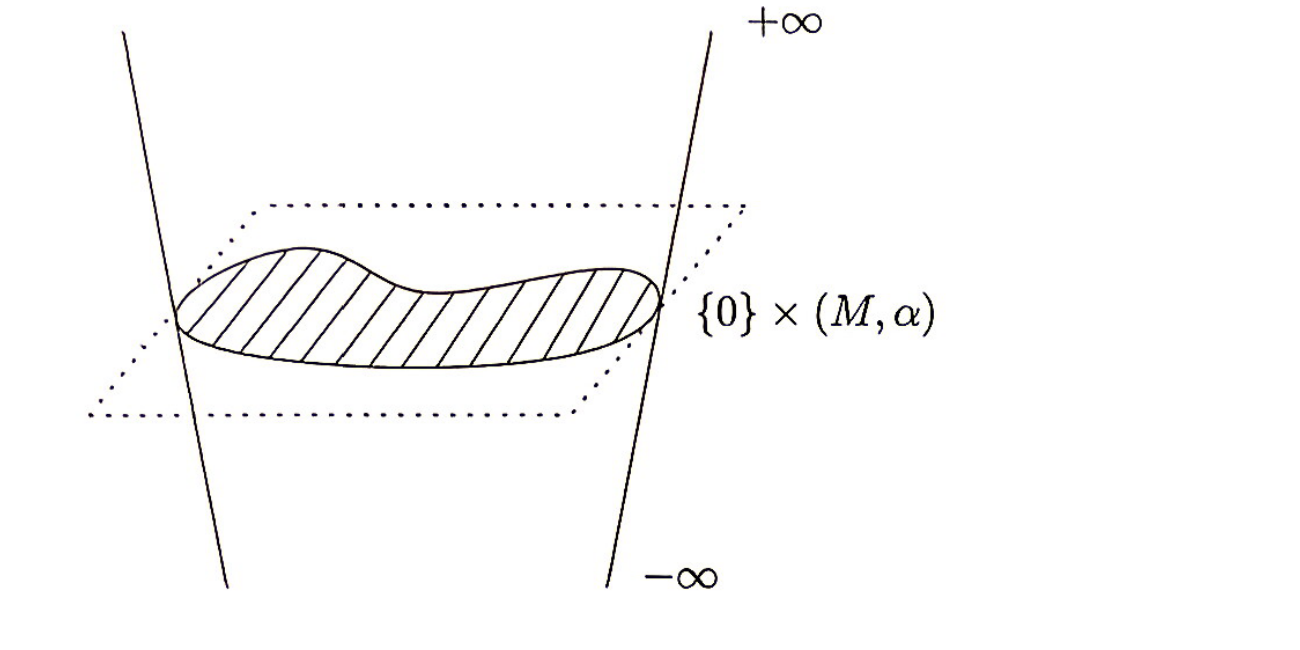
\includegraphics[width=0.44\linewidth]{figures/fig_p070_1.png}
  \caption*{图 3.4\quad $(M,\xi=\ker\alpha)$ 的辛化
  （原书 p.62, Figure 3.4）}
\end{figure}

% [Tutor Note: 原文疑误——上式 $\dd\alpha(v,\eta)$ 中的 $v$ 是 $\partial_r$
% 方向的标量系数，按上下文应为 $\dd\alpha(w,\eta)$：由 (3.2) 及
% $\eta=R_\alpha$ 得 $\dd\alpha(w,R_\alpha)=0$，故结果恰为 $v\neq0$。
% 已记入 review_ch03.md。]

反方向上，有时也可以从辛流形出发「提升」出切触流形。

\begin{wdefn}{3.2.2}
设 $(W,\dd\lambda)$ 是恰当辛流形。其\textbf{切触化}（contactization）是指
如下定义的切触流形：
\begin{equation}\tag{3.16}
  CW:=\bigl(W\times S^1,\ \xi=\ker(\lambda+\dd\theta)\bigr),
\end{equation}
其中 $\theta$ 是 $CW$ 中 $S^1$ 分量的坐标。
\end{wdefn}

容易验证 $\lambda+\dd\theta$ 确为切触 $1$-形式，满足非退化条件 (3.1)。下面是
一个有意义的练习。

\begin{wexer}{3.2.1}
从恰当辛流形 $(W,\dd\lambda)$ 出发，设其 Liouville 流整体定义。首先按定义
3.2.2 考虑其切触化 $CW$（关于切触 $1$-形式 $\alpha$）。然后按定义 3.2.1 考虑
$CW$ 的如下辛化：
\[
  S_+(CW)=\bigl(\R_{>0}\times CW,\ \dd(r\alpha)\bigr),
\]
其中多出的分量为 $\R_{>0}$（这里辛结构取 $\dd(r\alpha)$，而非定义 3.2.1 中的
$\dd(\ee^r\alpha)$）。试证明 $S_+(CW)$ 辛同胚于乘积
$\bigl(W\times T^*_{>0}S^1,\ \pi_1^*\dd\lambda+\pi_2^*(\dd r\wedge\dd\theta)
\bigr)$，其中 $\pi_1,\pi_2$ 分别是到 $W$ 与 $T^*_{>0}S^1$ 的投影。该乘积有时
称为 \textbf{$(W,\dd\lambda)$ 的稳定化}（stabilization）。
\end{wexer}
